\section{页面布局}
\subsection{geomtry}
本模板采用geomtry宏包进行页面的设置,其中对如下的原始命令进行了重定义:
\begin{bytes}
\renewcommand{\newgeometry}[1]{
    \Gm@restore@org
    \Gm@initnewgm
    \Gm@newgmtrue
    \setkeys{Gm}{#1}
    \Gm@newgmfalse
    \Gm@process
    \ifnum\mag=\@m\else\Gm@magtooffset\fi
    \Gm@changelayout
    \Gm@showparams{newgeometry}
}
\renewcommand{\restoregeometry}{
    \Gm@restore@pkg
    \Gm@changelayout
    }
\end{bytes}

\clearpage
\subsection{margin}
由于\verb|\marginpar|命令采用\LaTeX{}的浮动机制实现,所以可能不紧邻对应的内容,于是我们采用更加稳定的
marginnote宏包提供的\verb|\marginnote|命令,基础命令格式说明:
\begin{verbatim}
\marginnote[<left content>]{<right content>}[<voffset>]
\end{verbatim}

% the left contents shows only when document class is 'twoside'
\marginnote{
    \begin{center}
        \tikz\draw[->] (0, 1) -- (2, 1);

        The First Margin(mandatory):
    \end{center}
}

\vspace*{6em}
可以在margin中绘制其他的tikz图形,但如果两个margin的距离等参数调整的不太合理时,\TeX{}就会丢出警告:
{
    \ttfamily
    Marginpar on page 1 moved.
}
\marginnote[-4em]{%
    \begin{center}
        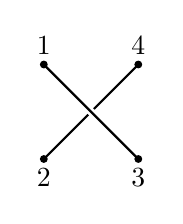
\begin{tikzpicture}[scale=.6]
            \draw[black,thick] (-1,-1) -- (-.06,-.06);
            \draw[black,thick] (.06,.06) -- (1,1);
            \draw[black,thick] (-1,1) -- (1,-1);
            \filldraw[black] (-1,-1) circle (2pt) node[anchor=north] {2};
            \filldraw[black] (-1,1) circle (2pt) node[anchor=south] {1};
            \filldraw[black] (1,-1) circle (2pt) node[anchor=north] {3};
            \filldraw[black] (1,1) circle (2pt) node[anchor=south] {4};
        \end{tikzpicture}
        
        一个tikz示意图
    \end{center}
}

本模板支持在特定页面取消margin,重新设置当前页面的布局,只需使用本模板提供的
\verb|\nomargin|命令即可。

同时本模板支持两种布局格式:
\begin{itemize}
    \item 带有margin的默认模式,margin的宽为1.5cm,位于页面的右侧,当然本模板仍提供了没有margin的\verb|nomarg|环境
    \item 取消margin的普通布局,需使用\verb|\nomargin|开启,使用\verb|\margin|结束,
        两者之间的内容为取消margin之后的页面布局,并且自动换页。如果忘记使用\verb|\margin|命令结尾的话,
        后续的页面布局中布局会乱排。
\end{itemize}

所以一定要养成良好习惯,前后命令成对书写\footnote[1]{注意:没有nomargin对应的局部环境}

\vfill 

\textcolor{red}{\thepage{}页底部}


% 使用\nomargin后会自动换页
\nomargin
\subsection{Margin测试}
使用\verb|\nomargin|后会自动换页,比如从这里的第\number\numexpr\value{page}-1页自动换到\thepage{}页:
\begin{bytes}
% 第一页内容 ...
\nomargin
\section{Margin测试}
使用\verb|\nomargin|后会自动换页,...

\section{脚注测试}
本模板还对footnote进行了相关的定制,...
\begin{itemize}
    \item footnote定制\footnote[1]{这是第一个脚注}
    \item footnote定制\footnote[2]{这是第二个脚注}
\end{itemize}
\margin
\end{bytes}

还有就是可以从下面的公式布局看出当前是否有margin,
\begin{align}
    \sum_{i=1}^{+\infty}{\int_{0}^{i}-\frac{1}{t}\mathrm{d}t} = \frac{\pi^2}{6}
\end{align}


\subsection{Margin With FootNote}
本模板还对footnote进行了相关的定制,使用\verb|\footnote|命令,会自动将脚注编号添加到脚注内容上。设置了
footskip等值,使用效果如下:
\begin{itemize}
    \item footnote定制\footnote[1]{这是第一个脚注}
    \item footnote定制\footnote[2]{这是第二个脚注}
\end{itemize}
\vfill 

\textcolor{red}{\thepage{}页底部}
\margin
